\chapter{Introduction and background}
\label{chap:intro}

PrankWeb is a web-based tool for predicting ligand-binding sites for a given protein structure. PrankWeb uses a tool called P2Rank for the prediction of binding sites on the backend. In this thesis, an improved version of PrankWeb is introduced, with an emphasis on the modernization of the frontend and creating a potential for implementing post-processing features, such as docking.

In this chapter, we will discuss the basics of protein and ligand-binding sites problematic to get briefly acquainted with the topic. A short intro to the used data formats in this thesis will follow. Later in this chapter, we will cover the current PrankWeb architecture and the P2Rank tool itself to get a better understanding of the project. The reader will also be briefly introduced to similar web tools for the prediction of ligand-binding sites.

\section{Introduction to molecular biology}
\label{sec:mol_bio}

In this section, we will briefly introduce the basics of molecular biology. We will focus on the protein structures and their interactions with other molecules. The reader is assumed to have a basic knowledge of protein structures and this terminology to understand the concepts of the entire thesis.

\subsection{Amino acids and proteins}
\label{subsec:amino_acids}

\textbf{Amino acids} are in general molecules containing an amino group (-NH$_2$), a carboxyl group (-COOH), and a R group (also called side chain). Although there are hundreds of known amino acids, 20 of them provide the key to the structure of thousands of different proteins. In this thesis, we will focus on the 20 proteinogenic amino acids that are used in the protein structures. Amino acids are the building blocks for proteins that serve as diverse products, such as enzymes, hormones, antibodies, muscle fibers, transporters, and many more.

\textbf{Proteins} are polymers consisting of a linear chain of amino acids. Each of the so-called \textbf{amino-acid residues} is connected to its neighbor by a covalent bond. The connected amino acids form a \textbf{chain}. Proteins are occurring in all cells and all parts of the cells. Proteins are the molecular instruments through which genetic information is expressed. Cells may produce proteins with substantially different properties and activities just by joining them in a different \textbf{sequence} (also called \textbf{primary structure}). The 3D protein representation based on a sequence of the protein's amino acids is called the \textbf{tertiary structure} \cite{nelson2008lehninger}.

Billions of proteins are known by their sequence, but only a small fraction of them are known by their tertiary structure. The structures may be determined by experiments, we call these structures \textbf{experimental}. Despite the effort to determine the structures, the vast majority of actual protein structures remain unknown. Nowadays, various tools are used for predicting unknown structures. A notable example is a neural network called AlphaFold that allows the prediction of a protein structure based on its sequence by assigning a probability to each amino acid in the sequence (called pLDDT). We refer to these structures as \textbf{predicted} \cite{jumper2021highly}.

\subsection{Protein functions}
\label{subsec:protein_functions}

The functions of proteins depend not only on the protein structures but also on the environment in which they are located. Many protein functions are involved by the reversible binding to other molecules. A molecule that is reversibly bound to a protein is called a \textbf{ligand} (also \textbf{protein ligand}). A ligand may be any kind of molecule, including another protein, or a small molecule.

One ligand binds on a part of the protein surface. This is called the \textbf{ligand-binding site}. This binding is not only defined by its molecule, but also by other properties such as shape, size, and charge. We refer to the binding site as a \textbf{pocket} \cite{nelson2008lehninger}.

In PrankWeb, the main focus is to create a \textbf{prediction} of the potential locations and interacting residues of small molecule ligands for a given protein structure. 

These predictions may or may not be based on various physical and chemical properties of spots on the protein surface, and \textbf{evolutionary conservation} score of the residues. The conservation score is a measure of how similar the residues are in different protein structures. In PrankWeb, evolutionary conservation is explicitly visualized.

One of the PrankWeb extensions is the possibility to \textbf{dock} a ligand to a binding site. Docking is a complex process of computing the mutual positions of the ligand and the protein structure. This computation also provides information about the potential energy of the protein-ligand complex. This altogether allows us to predict the potential of real-life binding of the ligand to the protein structure \cite{sulimov2019advances}.

\section{Used data formats}
\label{sec:used_data_formats}

PrankWeb uses several data formats for the input and output of data throughout the application. In this section, we will briefly introduce the used data formats.

\subsection{JSON}
\label{subsec:json}

JSON (JavaScript Object Notation) is a data format used for storing JavaScript objects. The syntax of this format is simple and the main advantages of this format are its readability and simple usage on the frontend. The main idea of JSON is to store its data in key-value pairs. The keys are strings and the actual values may be in any format such as string, number, boolean, array, or another object.

\begin{lstlisting}[language=JavaScript,caption={
    An example of a JSON file used for storing information about the prediction for the 2SRC protein structure.
}]
{
    "id": "2SRC",
    "database": "v3",
    "created": "2023-02-25T20:58:07",
    "lastChange": "2023-02-25T20:58:26",
    "status": "successful",
    "metadata": {
        "predictionName": "2SRC",
        "structureName": "structure.cif"
    }
}
\end{lstlisting}


\subsection{PDB}
\label{subsec:PDB}

PDB (Protein Data Bank format) is a file format that is used for describing three-dimensional protein structures. This format stores information about the atom coordinates and their connections \cite{bernstein1977protein}. Alongside this information, the PDB format may contain additional metadata as well. It is still used for many protein structures, but the format size is limited and thus it does not support large structures, so in some cases, it is replaced by the PDBx/mmCIF format (\cref{subsec:PDBx_mmCIF}) \cite{adams2019announcing}. A large database of PDB files for protein structures is called RCSB PDB\footnote{PDB database is available at \url{https://www.rcsb.org/}.}.

\lstinputlisting[caption={
    An edited example of a PDB file used for storing information about the 2SRC protein structure.
}]{code/2src.pdb}


\subsection{PDBx/mmCIF}
\label{subsec:PDBx_mmCIF}

PDBx/mmCIF (Protein Data Bank extended / macromolecular Crystallographic Information File) is an extension to the CIF format that stores crystallographic data. It was developed to overcome the limitations of the existing formats \cite{bourne199730}.

\subsection{FASTA}
\label{subsec:FASTA}

FASTA (FAST-All) is a text format that describes either a nucleotide sequence or a protein sequence. In our case, this format is used in the second sense. This format is simple as it only contains a brief description of the protein on the first line starting with the ">" character and the sequence itself on the next line. The sequence is represented by a string of letters that represent the amino acids. This format was created for the FASTA program that was used for sequence alignment \cite{lipman1985rapid}.

\begin{lstlisting}[caption={
    An example of a FASTA file used for storing information about the 7VNU sequence.
}, breaklines=true, breakatwhitespace=false,escapechar=*]
>7VNU_1|Chains A, B, C, D|Nucleoprotein|Severe acute respiratory syndrome coronavirus 2 (2697049)
GASNNTASWFTALTQHGKEDLKFPRGQGVPINTNSSPDDQIGYYRRATRRIRGGDGKMKDLSPRWY FYYLGTGPEAGLPYGANKDGIIWVATEGALNTPKDHIGTRNPANNAAIVLQLPQGTTLPKGFYAE
\end{lstlisting}

\subsection{CSV}
\label{subsec:CSV}

CSV (Comma-Separated Values) is a text format that is used for storing tabular data in plain text. The first line of the file contains the column names and the following lines contain the actual data. The data are separated either by commas or semicolons. This format is simple and easy to use, but it does not support complex data types such as arrays or objects.

\section{P2Rank tool}
\label{sec:p2rank}

P2Rank allows its users to predict the ligand-binding sites for a given protein. In contrast to other projects, P2Rank was one of the first tools to employ machine learning for predicting pockets. Most of the other tools use geometry-based, energetic-based, or template-based methods. P2Rank outperforms most of the existing binding sites prediction tools \cite{krivak2018p2rank}. Moreover, P2Rank works as a standalone application and is fully automated, which makes the tool very intuitive and easy to use.

P2Rank works with specific file formats such as PDB and PDBx/mmCIF. After running the tool on a specific protein structure file, the tool will provide a CSV output file with the prediction and residue-level scores. The output file includes predicted pockets, their ranks, center coordinates, adjacent residues, related surface atoms and a probability score.

The tool was written in Java and requires only the JRE\footnote{Java Runtime Environment.} to run. Additionally, the source codes are publicly available at GitHub\footnote{Source codes for P2Rank are available at \url{https://github.com/rdk/p2rank}.}. This allows the users to potentially modify the tool to their respective needs. 

\section{PrankWeb architecture}
\label{sec:prankweb_arch}

PrankWeb consists of several components that cooperate together. Currently, the application is deployed via Docker\footnote{Docker is a virtualization tool providing a stable interface for isolating and running applications. More information is available at \url{https://www.docker.com/}.} containers that are described in the Docker-compose configuration file. The application consists of the following components:

\begin{itemize}
    \item \textbf{gateway} - a reverse proxy that is responsible for routing the requests to the respective backend services and for serving the frontend
    \item \textbf{rabbitmq} - a broker that is used for communication between the web server and the backend services
    \item \textbf{flower} - a tool for monitoring the RabbitMQ broker and Celery workers
    \item \textbf{web-server} - a Flask server responsible for communication between the gateway and the RabbitMQ broker
    \item \textbf{executor-p2rank} - a backend service that is responsible for running the P2Rank tool, employs Celery workers
    \item \textbf{executor-docking} - a backend service that is responsible for running the docking tool, employs Celery workers
    \item \textbf{prometheus} - a tool for monitoring the Docker containers 
\end{itemize}

\begin{figure}
    \centering
    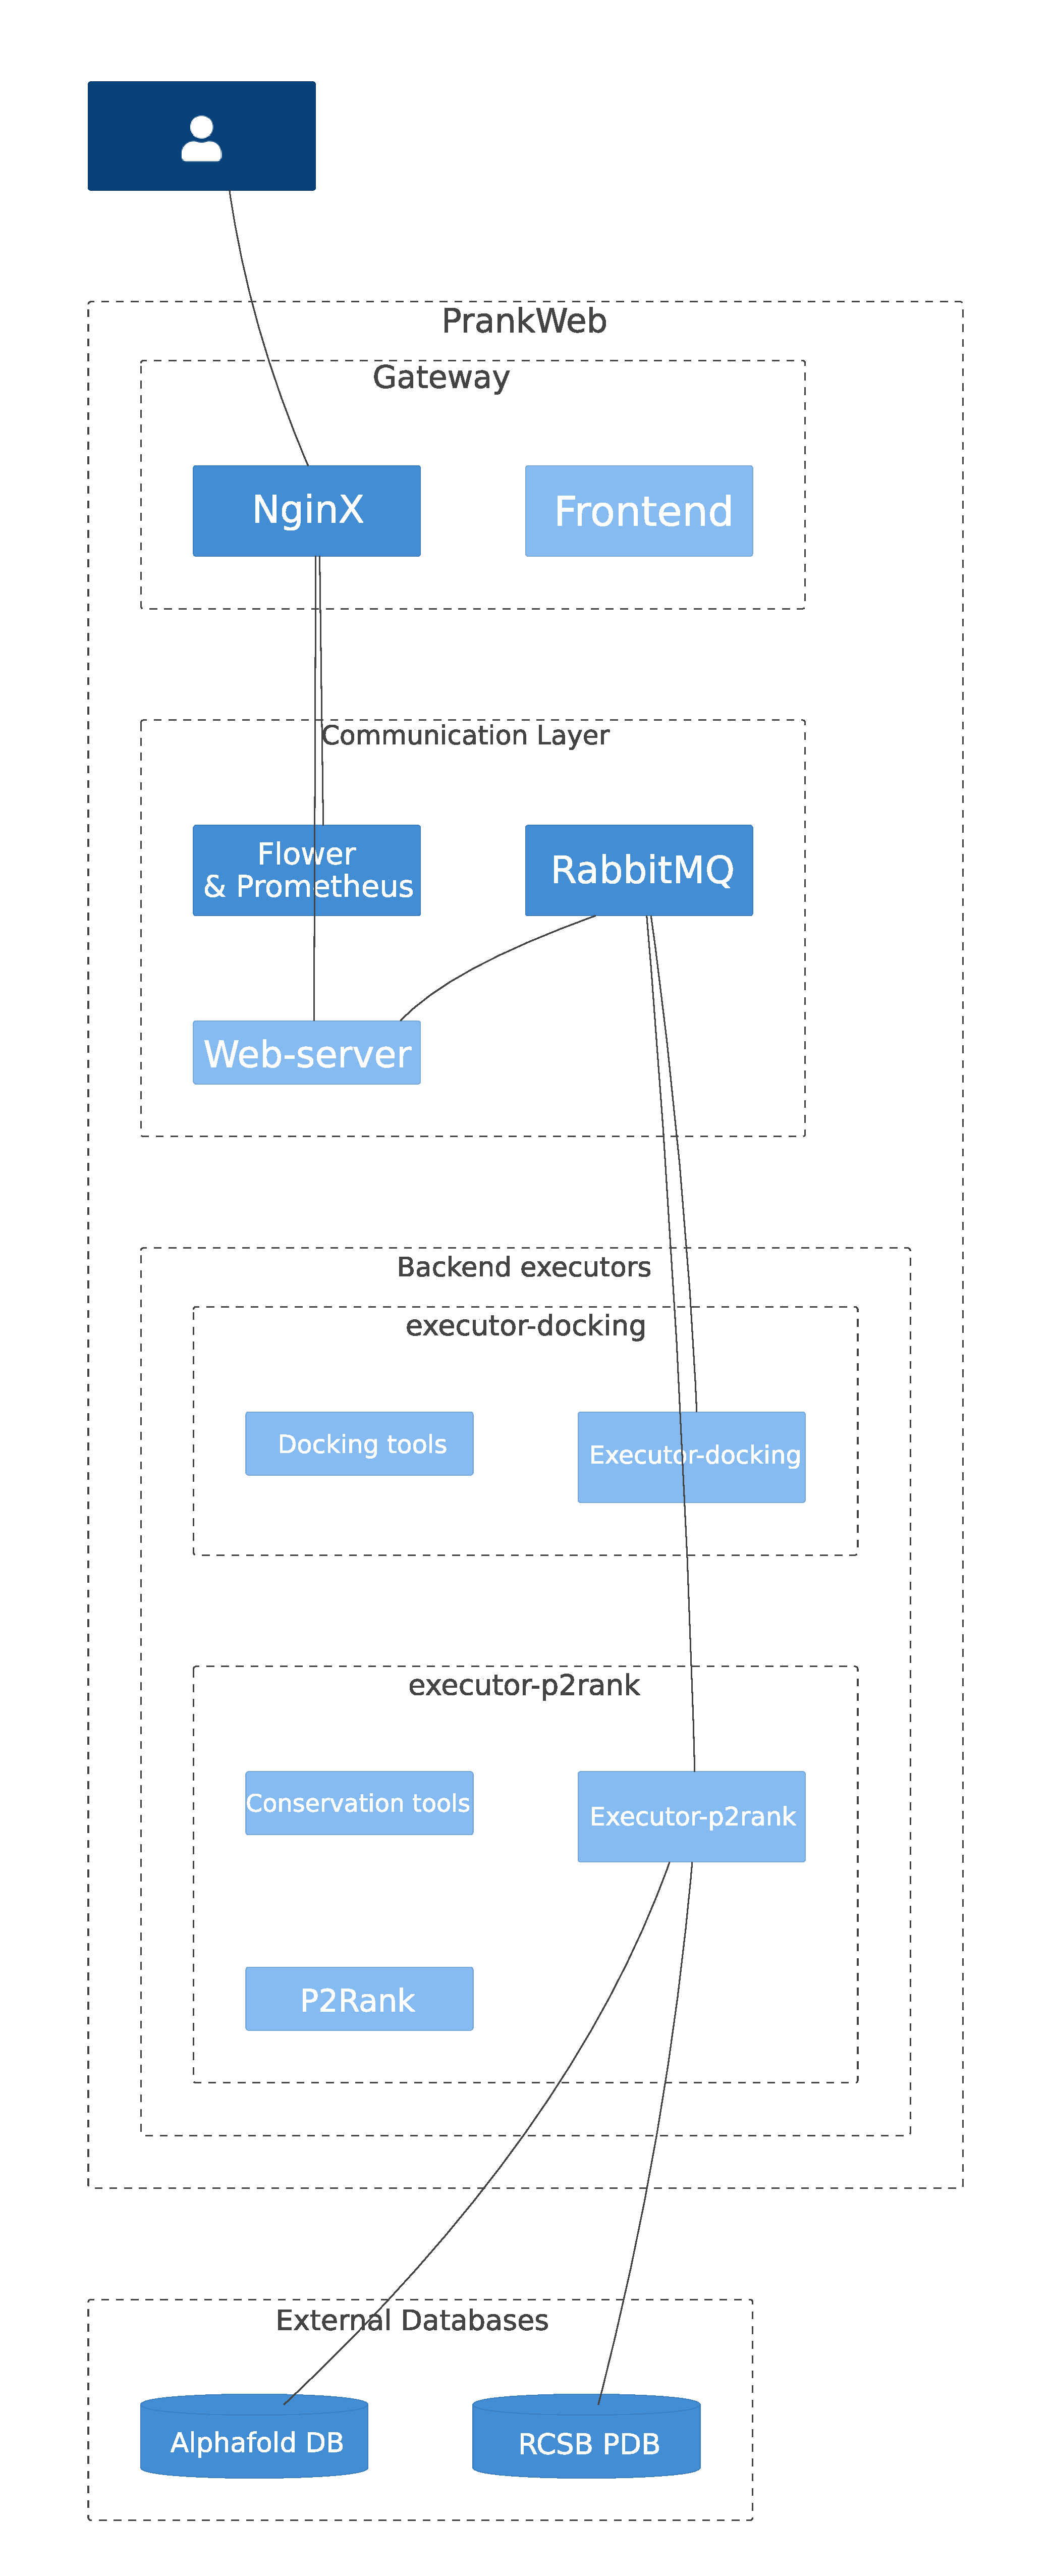
\includegraphics[height=0.95\textheight]{img/architecture.pdf}
    \caption{A simplified C4 model of the PrankWeb architecture.}
    \label{fig:architecture}
\end{figure}

A diagram of the architecture is shown in \cref{fig:architecture}. This diagram is a simplified version of the C4 model \cite{vazquez2020c4} for PrankWeb, dark blue boxes represent the containers, light blue boxes represent the components, and the arrows represent the communication between the services. For the completed C4 model with more details, see the original wiki page\footnote{The original wiki page is available at \url{https://github.com/cusbg/p2rank-framework/wiki/PrankWeb-architecture}}. The diagram includes retrieving information about the structures from external databases from AlphaFold \cite{david2022alphafold} and RCSB PDB \cite{kouranov2006rcsb}.

Some of the containers include environment variables that are required for the proper functionality. The environment variables are specified in the docker-compose configuration file. The user may modify these also by creating a \texttt{.env} file in the root directory of the project.

The docker-compose configuration file thus contains the entire PrankWeb logic. When employing a new plug-in or a new feature, a container may be introduced to this file to get easily integrated into the application.

Each of the containers is defined by a respective \texttt{Dockerfile}. Some containers are dependent on the order of deployment, some containers include a Docker volume definition that ensures the persistence of the data.

Now we will present the current Docker containers in more detail to get a broader knowledge of the architecture.

\subsection{Gateway}
\label{subsec:gateway}

The gateway container is a reverse proxy that is responsible for routing the requests to the backend. In PrankWeb, we utilize Nginx\footnote{Nginx is a web server used for serving static HTML content and acts as a reverse proxy. More information is available at \url{https://www.nginx.com/}.} as a reverse proxy. The Nginx configuration file is located in the \texttt{gateway/nginx.conf} file. The server configuration includes not only the reverse proxy routes but a mapping to the Flower and Prometheus services as well.

Moreover, \texttt{gateway/Dockerfile} is responsible for the installation of the frontend. The frontend is a React\footnote{React is a library for creating modern and intuitive user interfaces for web browsers. More information is available at \url{https://react.dev/}.} application built via webpack\footnote{webpack is a module bundler used to bundle JavaScript for web browsers. More information is available at \url{https://webpack.js.org/}.}. PrankWeb utilizes two main external libraries for the bioinformatic part of the application, MolStar and RCSB Saguaro Feature 1D Viewer. We will discuss these libraries in more detail in \cref{sec:frontend}.

The entire frontend is written in TypeScript, JavaScript, CSS, SCSS, and HTML.

\subsection{RabbitMQ}
\label{subsec:rabbitmq}

RabbitMQ\footnote{More information about RabbitMQ is available at \url{https://www.rabbitmq.com/}.} is a message broker that is used to provide communication between the web server and the backend workers, in our case Celery. RabbitMQ is configured via the respective configuration file. PrankWeb does not require a complex configuration of this service, although the service is still necessary for communication.

\subsection{Flower}
\label{subsec:flower}

Flower\footnote{Source codes for Flower are available at \url{https://github.com/mher/flower}.} is a tool for monitoring the broker and Celery\footnote{Celery is a distributed task queue for Python. This allows the users to distribute given tasks around multiple workers (in our case threads), so multiple tasks may run in parallel. Source codes are available at \url{https://github.com/celery/celery}.} workers' functionality. The Flower container does not need any specific configuration, it is only necessary to correctly run it alongside the RabbitMQ container.

\subsection{Web-server}
\label{subsec:web-server}

The web-server container is a WSGI server that is responsible for serving the web application. Currently, we employ the Gunicorn\footnote{More information about Gunicorn is available at \url{https://gunicorn.org/}.} server. The second main part of this container is Flask\footnote{Flask is a micro-framework for Python used for creating simple web applications. Source codes are available at \url{https://github.com/pallets/flask}.} framework. The Flask application defines all of the REST API endpoints for interaction between the frontend and the backend. This application also defines a Celery client that is responsible for sending the tasks to the backend Celery workers based on the API calls.

\subsection{Executor-P2Rank}
\label{subsec:executor-p2rank}

This container is responsible for creating the prediction via the P2Rank tool. P2Rank executor is written in Python and utilizes the Celery framework for task management. Celery enables the server to use multiple threads and process the requests in parallel. The executor's Celery listener first receives a request for the prediction given a directory with the name of the structure. Subsequently, the executor prepares the necessary information for the P2Rank tool.

The tool is then run and the results are saved in the

\texttt{predictions/<db-name>\footnote{Represents the current version of database such as v2, v3, v3-alphafold, v3-conservation-hmm etc.}/<structure-short>\footnote{The shortcut consists of second two letters of the structure identifier, i.e \texttt{SR} for \texttt{2SRC} or \texttt{5V} for \texttt{Q5VSL9}.}/<structure-name>} 

directory. The current hierarchy contains the following:
\begin{itemize}
    \item \texttt{input/configuration.json} - a JSON file required for a configuration of the P2Rank tool, containing the structure code, name of the structure file, conservation and others
    \item \texttt{public/structure.cif.gz} - a gzipped\footnote{Gzip is an Unix-based tool for file compression.} mmCIF/PDB file of the structure
    \item \texttt{public/prediction.json} - a JSON file containing the prediction results derived from the P2Rank tool specifically for easier parsing in the frontend
    \item \texttt{public/prankweb.zip} - a zip file containing unmodified, verbose output files directly from the P2Rank tool
    \item \texttt{info.json} - a JSON file containing current prediction status
    \item \texttt{log} - a log file containing the output of the P2Rank tool
\end{itemize}

All of the listed files are exposed via the REST API to the frontend. After posting a prediction request, the frontend periodically polls the \texttt{info.json} file to get the current status of the prediction. Meanwhile, the \texttt{log} file is continuously updated with the output of the P2Rank tool. The log file is also shown in the frontend to provide the user with the current status of the prediction.

\subsection{Executor-Docking}
\label{subsec:executor-docking}

This container is responsible for the docking backend task. More information about the docking task is available in \cref{subsec:server-side-plugins}.

\subsection{Prometheus}
\label{subsec:prometheus}

Prometheus\footnote{More information about Prometheus is available at \url{https://prometheus.io/}.} is a tool for monitoring the Docker containers. It is not necessary for the proper application functionality but is useful for debugging purposes. The Prometheus container is configured via the respective configuration file. The interface is exposed at the \texttt{9090} port.

\section{Similar web-tools}
\label{sec:similar_web_tools}

The main motivation for the creation of PrankWeb was to provide a web-based ligand binding site prediction tool that employs the newest technologies. One of the goals of this thesis is to replace the outdated plugins for the structure and binding site visualization to keep the application relevant and up-to-date.

There are a few working web tools that can predict binding sites for the structure as well. The main issue with these tools is that most of them are utilizing outdated technologies and do not appear to be as intuitive as PrankWeb\cite{jendele2019prankweb}. Moreover, PrankWeb focuses on the visual side of the prediction and provides a more detailed view of the results, while the other tools are relying on the user to interpret the downloadable results in other tools such as PyMOL.

We will cover a few of the existing web tools to provide a better understanding of some of the existing solutions for the ligand binding site prediction which are currently available.

\subsection{IntFOLD}
\label{subsec:intfold}

IntFOLD\footnote{Available at \url{https://www.reading.ac.uk/bioinf/IntFOLD/}.} is a tool that may be used for predicting protein tertiary structures alongside disordered protein regions and ligand binding sites. This tool utilizes the FunFOLD algorithm to create the predictions effectively \cite{10.1093/nar/gkz322}. IntFOLD appears to be still actively developed and is easily accessible to any potential user. The user interface is easy to use and requires only the protein sequence (FASTA) to be entered. On the other side, IntFOLD uses the JSMol library for visualizing the protein binding sites. JSMol is more of a simple viewer with fewer options than the LiteMol library used in PrankWeb. Both the visuals and the user interaction are limited. The user may modify the representation with a right mouse button click, but the interface is pretty complicated and non-intuitive. An example prediction is shown in Figure \ref{fig:intfold_prediction}. Like PrankWeb, IntFOLD also provides a download option for the prediction results for PyMOL. The prediction takes a long time to be computed, typically around 24 hours.

\begin{figure}
    \centering
    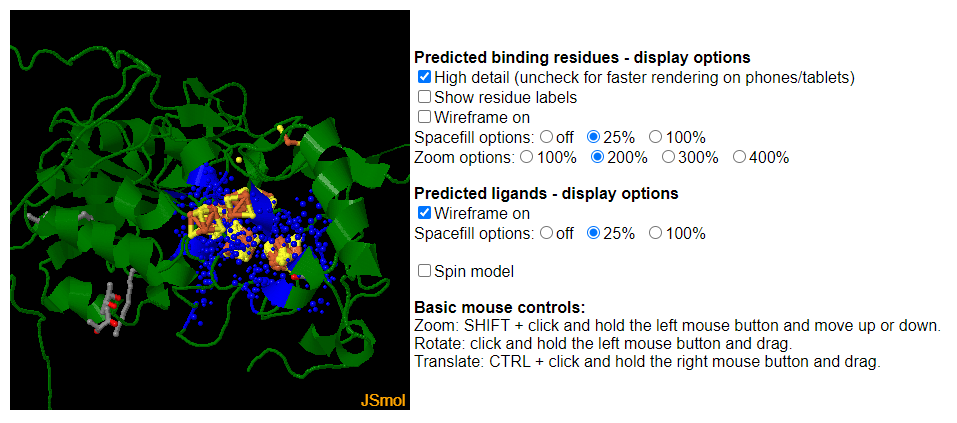
\includegraphics[width=\linewidth]{img/intfold_prediction.png}
    \caption{JSmol view of ligand binding residues prediction for T1114s2.
    Available at \url{https://www.reading.ac.uk/bioinf/servlets/nFOLD/IntFOLD7results.jsp?time=17_8_50_25_11-5-2022_CASP_ALL_mesu41b7re376c8l&md5=mesu41b7re376c8l&targetname=T1114s2}. The structure is shown in dark green, the binding sites prediction is shown in blue. Predicted ligands are shown yellow-orange. Available as a sample prediction from IntFOLD.}
    \label{fig:intfold_prediction}
\end{figure}

\subsection{COACH}
\label{subsec:coach}

COACH\footnote{Available at \url{https://seq2fun.dcmb.med.umich.edu/COACH/}} is a web-based tool designed specifically for binding site prediction, like PrankWeb. COACH uses a combination of substructure-comparison (TM-Site) and sequence-alignment (S-Site) methods for the computations of potential binding sites \cite{yang2013protein}. This combination of methods is generally slower than the machine learning method used in P2Rank, so the prediction once again is available to the user after a long time, typically around 24 hours. This tool allows the user not only to enter a FASTA sequence but also to upload or paste a PDB file. COACH allows the user to download the prediction results as well and does not focus on the very limited web visualization. An example prediction is shown in Figure \ref{fig:coach_prediction}.

\begin{figure}
    \centering
    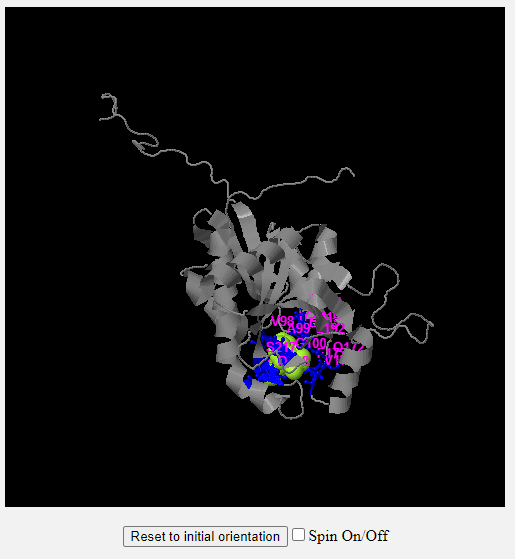
\includegraphics[width=.75\linewidth]{img/coach_prediction.png}
    \caption{JSmol view of a COACH prediction result for a sample protein available at \url{https://seq2fun.dcmb.med.umich.edu/COACH/CH000001/}. Compared to IntFOLD, the structure has implicitly fewer details and the user may change the representation only with a right mouse button click via JSMol settings.}
    \label{fig:coach_prediction}
\end{figure}

\subsection{DeepSite}
\label{subsec:deepsite}

DeepSite\footnote{Available at \url{https://www.playmolecule.com/deepsite/}} is one of the newest tools for predicting binding sites. DeepSite is a part of the PlayMolecule framework that aims at the visual representation of the protein structures and their interactions in a user-friendly web interface \cite{martinez2017playmolecule} \cite{10.1093/bioinformatics/bty758}, which is highly applicable in computational drug discovery. DeepSite uses machine-learning-based methods to precisely predict the binding sites, which makes the tool very fast \cite{10.1093/bioinformatics/btx350}. The waiting times are significantly slower and the prediction is available to the user after a few minutes. The user may enter the PDB structure ID, which is a lot more convenient way to describe the structure than by entering the entire PDB file. On the other side, entering a custom format is a more generic way that does not limit the user to the existing PDB database. DeepSite utilizes the MolStar library for the results visualization and is similar to PrankWeb in terms of visual representation. On the other side, DeepSite provides the user only with a visualization of the center of the binding site and does not provide any information about the residues that are involved in the binding directly in the web viewer. The structure is shown in a surface representation. An example prediction is shown in Figure \ref{fig:deepsite_prediction}. The pros of this tool are definitely the speed of the prediction and an above-average visual representation. On the other side, the user is provided with little information about the binding site and may be used for a rather quick overview of the potential binding sites.

\begin{figure}
    \centering
    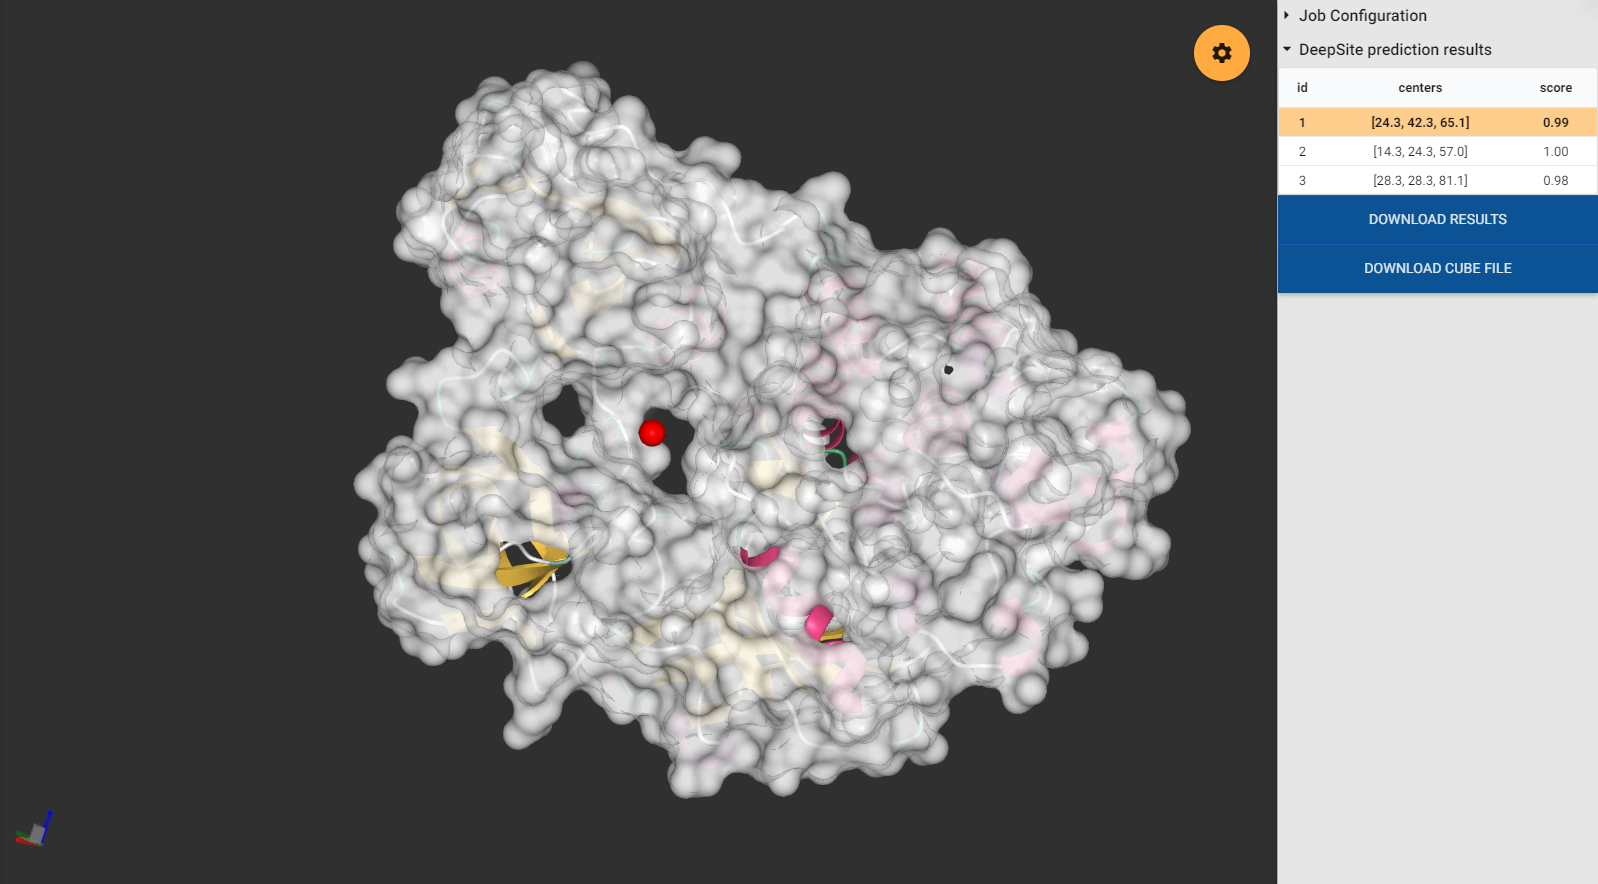
\includegraphics[width=\linewidth]{img/deepsite_prediction.png}
    \caption{A DeepSite prediction for the \texttt{2SRC} structure available at \url{https://www.playmolecule.com/deepsite/job/BD2ED307}. The surface representation is shown in white, underlying cartoon representation is colorful. The binding site prediction is shown by a red sphere.}
    \label{fig:deepsite_prediction}
\end{figure}